% The reading copy suppresses publisher metadata. A real submission ID selects review output.
\ifdefined\RealSubmissionID\else\PassOptionsToClass{nonacm}{acmart}\fi
\documentclass[acmtog,anonymous,review]{acmart}
\ifdefined\RealSubmissionID\acmSubmissionID{\RealSubmissionID}\fi
\citestyle{acmauthoryear}
\setcopyright{none}
\settopmatter{printacmref=false,printfolios=true}
\acmDOI{}
\acmJournal{TOG}
\title{Which Material Sites Can Stay Unlit After a Fire Edit?}
\author{Anonymous}
\begin{document}
\begin{abstract}
A second ignition stroke can move fire away from sites that burned in the original take as well as light new ones. We study a preview that answers a smaller, discrete question from a checkpoint of the edited simulation. Which currently unlit material sites can we guarantee will remain unlit over the next few frames? We enclose the motion of hot particles and the locations of possible births, then propagate an upper bound on heat through every ignition test. A site whose bound crosses the threshold remains undecided. In two orders of the same edit on a reconstructed woodpile, the weighted bound certifies 373,913 of 535,437 repeated site queries. An ordinary count of reachable carriers certifies 328,626. Both sets agree with native replay on every certified query. All 18 complete-domain queries still require replay. Restricting the query to the material immediately outside the second brush yields the same outcome, even in the eight windows with no ignition in that region. The gap between certifying sites and resolving an editing decision limits the case for interactive use.
\end{abstract}
\keywords{physics-based animation, simulation editing, ignition, conservative bounds}
\maketitle

\section{An edit with a signed footprint}
Consider a shot of a burning woodpile. After several seconds the editor adds another ignition stroke. Which material points burn differently at the end? An overlay of the stroke on the original take assumes the new fire cannot suppress a previous ignition. A shared gas budget and the order in which burning materials emit particles can break that assumption. On a reconstructed woodpile with 34,687 material splats we compare a single stroke with a second stroke added at frame 180. An ordinary global pool of particle slots allows the second group to emit. At frame 360 the second stroke has ignited 288 sites directly. Outside the stroke, 1,266 sites gain burning status and 12 lose it relative to the single-stroke take. Restricting admission to per-layer quotas eliminates the off-stroke change on this edit.

The first divergence in emitted gas under the global policy occurs at frame 205. Replaying the edited simulation through 150 of the 180 remaining frames recovers its endpoint burning set on this take. An editor cannot know this cutoff in advance. We investigate a narrower query that remains available after divergence. Given the \emph{current edited state}, report which unlit, fuel-positive sites will stay unlit in each of the next $H$ updates. A useful guarantee must survive the discrete ignition test at every update. A speed claim additionally requires that the guarantee save work for the output an editor requested.

\begin{figure*}[t]
\centering
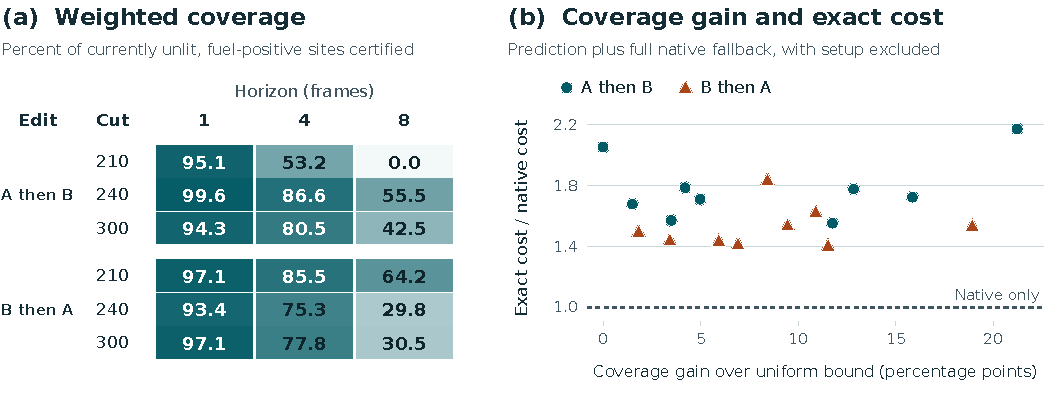
\includegraphics[width=\textwidth]{ignition-coverage.pdf}
\caption{Left, the fraction of eligible sites certified by the weighted rule on each edit and checkpoint. Right, each mark compares weighted with uniform coverage and the cost of weighted computation plus native fallback with direct native replay. Both costs start from the same edited state. The predictor cost excludes setup and output.}
\Description{Coverage generally falls with horizon, reaching zero at eight steps on the first edit's frame-210 cut. All eighteen measured cost ratios exceed one.}
\label{fig:coverage}
\end{figure*}

\section{Related work}
\citet{shen2026} synthesize combustion in Gaussian-splat scenes with volumetric simulation and rendering. Their results motivate the editing domain. We use exact labels from a particular discrete simulator as ground truth. Image realism and combustion fidelity require separate evaluation. \citet{chen2026} restrict fluid control to spacetime windows to revise an existing trajectory. Their optimization returns control forces. Our query returns one-sided decisions about a fixed edited trajectory. \citet{goel2022} support approximate spacetime queries over compressed ensembles of precomputed simulations. Here the future of the edited trajectory is unavailable when its labels are predicted.

\section{A sufficient condition for remaining unlit}
The material sites are fixed in world space. The solver advects gas particles on nine parallel layers and selects at most 160 hot carriers for material heating per step. Each selected particle of visual temperature $T$ at distance $d$ contributes $\Delta t\, aT(1-d/R)_+$, where $R=0.14$ and $a=2.2$. Material heat then decays and the solver tests for ignition. Heat arriving from the material graph after that test enters the next scan. Turning off intermediate renders preserves the discrete dynamics used here.

Let $u_i$ bound the current stored heat at a cold recipient $i$. For each future update $k$ compute an upper bound $F_{ik}$ on flame heat and $G_{ik}$ on graph heat. With $D=1-0.35\Delta t$, define
\begin{align}
  v_{ik} &= \mathrm{up}\bigl(D\,\mathrm{up}(u_i + F_{ik})\bigr),\\
  u_i &\gets \mathrm{up}(v_{ik}+G_{ik}).
\end{align}
Here $\mathrm{up}$ accounts for the number of nonnegative additions and the native binary32 stores. For at most $n$ writes the implementation inflates the sum of the initial value and the positive increments by a factor $1/(1-n2^{-24})$, with a per-write underflow allowance and a guard for binary64 reduction. This overestimate is applied separately at each phase. If every $v_{ik}$ remains below the native threshold of 1, induction over these phases certifies the site through $H$. A failed inequality leaves the site's future open.

For $F_{ik}$, group extant hot carriers by layer and a cell of width $R$. Retain the group's bounding box, particle count and largest visual temperature. Dilate its horizontal extent by the speed limit times elapsed time, with a margin for native velocity storage. Depth stays on the layer. A lower bound $d_{\min}$ on distance from the expanded group and an upper bound on its cooling temperature give an upper weight for each member. Sum the weights over reachable groups and cap by the sampled carrier count. For births we expand source boxes to include the solver's position jitter. A newborn first heats a recipient on a later step. We bound at most 48 offers per step. Where survival and the round-robin cursor establish a source's identity we bound its position directly. Once the cursor can wrap into an uncertain frontier, unlocated offers can heat anywhere. This is a deliberate loss of selectivity. For graph heating we use the serviced donor prefix if its fuel survives the horizon, or bound all possible serviced donations. These conditions limit the argument to the captured controls and native operator.

\section{Protocol and controls}
We ran two 360-step takes at 60 Hz with seed 11 on the Firewoods reconstruction distributed with \citet{shen2026}. The first ignites location A then B, the second B then A. The second stroke is applied between steps at frame 180. Both switch from per-layer to global admission at that intervention. The three checkpoints at frames 210, 240 and 300 and the horizons of 1, 4 and 8 steps were fixed before capture. The first take reproduces previously reconstructed ignition labels across every suffix frame. The reversed take produces a different endpoint with 8,427 burning sites, compared with 5,057 in the first. Reversing the strokes tests transfer across an edit order with shared scene, controls and seed. Both edits were defined by the researchers.

We compare four bounds using the same material graph and initial heat. The global bound allows all sampled carriers at every site. The support rule abstains whenever any possibly hot carrier can reach the site. The uniform rule counts reachable hot carriers with unit weight. The weighted rule adds temperature and radial attenuation. A separate evaluator compares the saved site IDs with all native ignition events over each horizon. Windows overlap and multiple queries may count the same site. The denominators below count site--window pairs, without implying independent trials.

\section{What the bounds decide}
\begin{table}[t]
\caption{Certified unlit site--window pairs. The warm and near-threshold columns are nested subsets, defined by positive initial heat and heat at least 0.5, respectively.}
\label{tab:mask}
\begin{tabular}{lrrr}
\toprule
Rule & All & Warm & Near threshold\\
\midrule
Eligible & 535,437 & 74,580 & 8,685\\
Global & 0 & 0 & 0\\
Gas support & 274,874 & 11,591 & 742\\
Uniform & 328,626 & 19,344 & 905\\
Weighted & 373,913 & 27,121 & 1,199\\
\bottomrule
\end{tabular}
\end{table}
The weighted rule gives 45,287 additional correct decisions over the uniform rule, including 294 near threshold (Table~\ref{tab:mask}). Of 1,108 observed ignitions counted across windows, all fell among the abstentions. Simply guessing that every initially cold site stays cold misses those 1,108 events. On the A-then-B cut at frame 210 the weighted rule certifies no sites at eight steps. After a potential cursor wrap, 218 offers have an unknown source across that horizon. Reversing the stroke order at the same frame certifies 19,432 sites at eight steps.

Figure~\ref{fig:coverage} shows how strongly coverage varies by checkpoint and horizon. Even when nearly all cold sites are covered, the remaining sites can determine the answer to an editor's question.

\section{Cost of an exact answer}
Native timing advances the gas and material without intermediate rendering and excludes recording per-site events. Starting from the in-memory edited cut, the median native time across 18 queries was 59.7 ms. The weighted predictor's median computation took 37.5 ms after preprocessing. All 18 windows contained undecided sites. Adding prediction and full-window native fallback gives a median of 92.8 ms, or a median paired ratio of $1.60$ relative to native replay. These quantities add separate measurements. They omit Python process startup, constructing the edited checkpoint, decoding it (20--43 ms per cut), preprocessing it (71--94 ms), and returning the masks. Shared transformed geometry took 7.4 ms to prepare. A live editor could amortize some of these costs across queries at the same checkpoint. That saving does not alter the need for fallback on the measured masks.

\subsection{Will the fire leave the second brush?}
We tested a region selected by the original stroke, where a single yes or no could inform an edit. Around the second brush of radius 0.12 we use the immediately adjacent shell, out to radius 0.26, one flame interaction radius beyond the brush. Does any currently cold site in this shell ignite within the window? The center follows the second stroke in each take. The rule, all cuts, and all horizons were fixed before regional scoring. The same two trajectories were reused. A native evaluator can stop on the first regional ignition.

All 18 queries were nonempty. Ten contained an ignition and eight did not. For this query the weighted rule certified 8,816 individual site--window pairs. Unit weights certified 6,537. Every window still contained an undecided site, including all eight with no ignition. At frame 240 of the first take, for example, the weighted rule certified 1,842 of 1,863 sites through the next scan. None ignited. The 21 unresolved sites nevertheless prevented an early answer. All 54 region-specific ID sets exactly matched the restrictions of their full-domain counterparts. Region-specific evaluation and native fallback together cost a median paired $1.40\times$ the ordinary first-event-or-end replay, starting with the checkpoint loaded; including file decoding increased this ratio to $3.05\times$. The native stepping component had a median of 17.7 ms. These additive costs use an optimistic native first-event cutoff from the trace and exclude an integrated interface.

We then tested two cheap ways to certify a positive answer on the same regions: enough residual heat to ignite at the next scan, and a lower bound on future heating from guaranteed surviving graph donors. The regional outcomes were already known when this follow-up was designed. Both rules abstained on every window, including the ten positives. A surviving donor prefix was available in all twelve multistep windows. This result bounds what these particular witnesses resolve; an ignition not proved by them cannot be assigned a causal source on that basis.

\balance
\subsection{Where the ordinary replay can stop}
We instrumented a fresh pair of continuous native takes to timestamp completion of the ignition scan within a step. Earlier steps must complete to provide the next state. The terminal step's graph, fuel and emission tail is needed only if the state must continue. Within the same execution, the median time for complete label queries was 71.8 ms through the full terminal step and 64.9 ms through its scan (median paired ratio 0.896). For the regional question, stopping at the first in-shell event or the horizon end, the corresponding medians were 18.6 and 11.85 ms (paired ratio 0.637). All recorded frame events agreed with the uninstrumented-by-this-timer reference. The timer measures prefixes of ordinary computation. A callable early-return implementation would also pay for dispatch, materializing the result and testing regional membership. These single-host paired comparisons use a separate run from the 17.7 ms regional timing above.


\section{Scope and open problems}
The evidence supports the feasibility of conservative material labels after gas divergence. Demonstrating an editing tool requires an output for which a partial answer has value, or an exact query the bound can decide more cheaply than native execution. The short windows here cover at most 133 ms of simulated time. They do not recover the full three-second revision from the second click. A single asset, one seed and two staged edits leave performance on other geometries, stochastic runs and creator-selected revisions open. The measurements do not establish a perceptual improvement. The terminal-scan timings supply a cost target for a future editor. A new method would need to return a correct regional answer, including useful positive witnesses near the advancing front, before a comparable native query completes.

\paragraph{Use of generative tools.}
OpenAI Codex agents helped design the hypotheses and protocols, implement the tests, analyze the results, review the method and draft the text. The counts come from the recorded simulation and scoring code.

\bibliographystyle{ACM-Reference-Format}
\bibliography{references}
\end{document}
